\documentclass[a4paper,10pt]{report}
\usepackage[utf8]{inputenc}
\usepackage{amsmath,amsfonts,amssymb}
\usepackage[margin=2cm]{geometry}
\usepackage{indentfirst}
\usepackage{subcaption,graphicx,float}
\usepackage{todonotes}

% Title Page
\title{Interpolation of Discretized Data}
\author{Milos Micik}


\begin{document}
\maketitle

\begin{abstract}
\todo{Add abstract}
\end{abstract}

\chapter{Introduction}
\todo{Add introduction.}

\chapter{Interpolation in 1D}
In one dimensional interpolation we have decided to compare interpolation methods using Bezier curves and cubic polynomial splines. Both methods use piecewise polynomials to trace a curve defined by knot points and information about the first derivatives.

\todo{Possibly add a bit of theory to splines.}

In 1D, the interpolation task is nearly straightforward. The only issue that can arise is when the data to be interpolated is discretized. This could occur for example when collecting data from a measurement where the measuring device has a finite precision and can only detect change in the observed quantity in steps.
\begin{figure}[h]
 \centering
 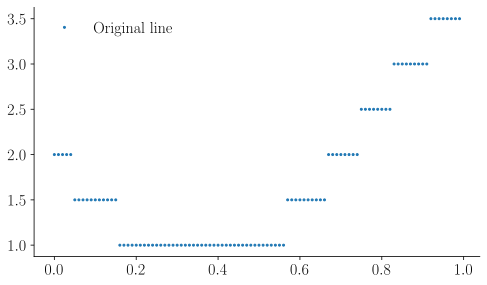
\includegraphics[width=.6\textwidth]{../images/1D_Function.png}
 % 1D_Function.png: 800x450 px, 100dpi, 20.32x11.43 cm, bb=0 0 576 324
 \caption{An example of discretized 1D data.}
 \label{fig:1D_fun}
\end{figure}

If we were to run the interpolation on such data without any adjustments, the polynomials would try to fit every single point in the collinear segments, producing a curve not too different from what we started with. Therefore in this case pre-processing of the data is required.

The pre-processing we have chosen assumes that the discretized data is obtained by rounding the real-data observation. For example, in Figure \ref{fig:1D_fun}, the collinear segment from $x\approx0.15$ to $x\approx0.55$ is represented in the data with $y$ value $1.0$, however by our assumption we know that the real values could have been anywhere in the interval $[0.75, 1.25)$. The pre-processing algorithm simply isolates a midpoint from a collinear region of points. Where the collinear region is a local maximum or minimum, we isolate two point instead, $1/3$ and $2/3$ along the collinear segment.

Using this algorithm, we can now interpolate any discretized curves in 1D. An example of it working in action can be seen in Figure \ref{fig:1D_fun_interpolated}:
\begin{figure}[H]
    \centering
    \begin{subfigure}{0.6\textwidth}
        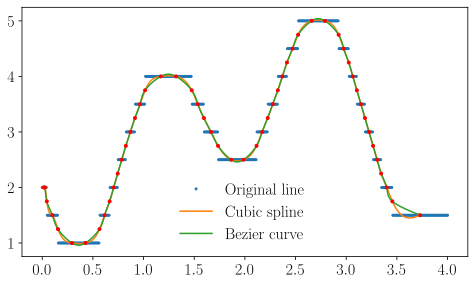
\includegraphics[width=\textwidth]{../images/1D_Function_Interpolated.png}
        % 1D_Function_Interpolated.png: 800x450 px, 100dpi, 20.32x11.43 cm, bb=0 0 576 324
    \end{subfigure}
    \hfill
    \begin{subfigure}{0.39\textwidth}
        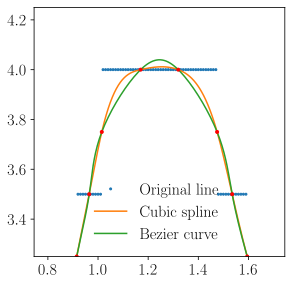
\includegraphics[width=\textwidth]{../images/1D_Function_Interpolated_Zoomed.png}
        % 1D_Function_Interpolated_Zoomed.png: 800x450 px, 100dpi, 20.32x11.43 cm, bb=0 0 576 324
    \end{subfigure}
    \caption{An example of curves interpolated from discretized 1D data.}
    \label{fig:1D_fun_interpolated}
\end{figure}

Note the subtle difference between the Bezier curve and the cubic spline. In segments which are relatively straight, their shape is very similar. However, the difference at places where the curve takes sharper turn is more noticeable. The cubic spline seems to achieve much better results, introducing less irregularities and copying the original data curve more smoothly. This does not come as a surprise, as cubic splines are expected to have \textit{$C^2$} continuity, whereas Bezier curves are only \textit{$C^1$} continuous.

\chapter{Interpolation in 2D}
\section{Parametric Curves}
Interpolating parametric curves in 2D (technically in any dimension) is very similar to interpolating in 1D. It might require different functions when implementing these in a programming language, but the algorithm is the same - if the data is discretized, we need to first isolate points from collinear segments.
\begin{figure}[H]
    \centering
    \begin{subfigure}{0.49\textwidth}
        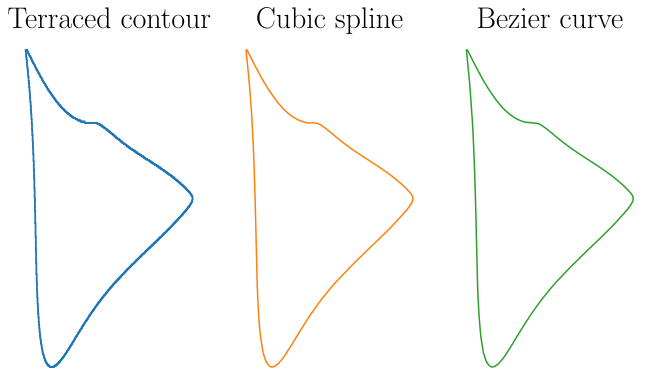
\includegraphics[width=\textwidth]{../images/2D_Contour.png}
    \end{subfigure}
    \hfill
    \begin{subfigure}{0.49\textwidth}
        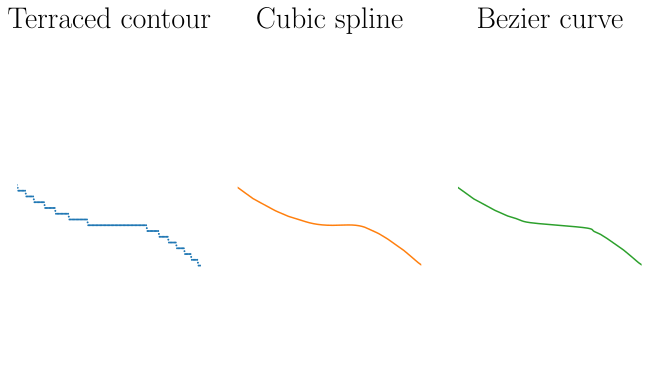
\includegraphics[width=\textwidth]{../images/2D_Contour_Zoomed.png}
    \end{subfigure}
    \caption{An example of parametric curves interpolated from discretized parametric 1D curve in 2D.}
    \label{fig:2D_parametric_curve}
\end{figure}

The same observation about the continuity holds in this case - cubic splines produce curves which look more natural.

\section{Countour lines}
Interpolating contour lines of 2D functions can be done by representing the contours as parametric curves. As an example, we will use digital elevation maps of regions from Scotland.



\begin{figure}[H]
 \centering
 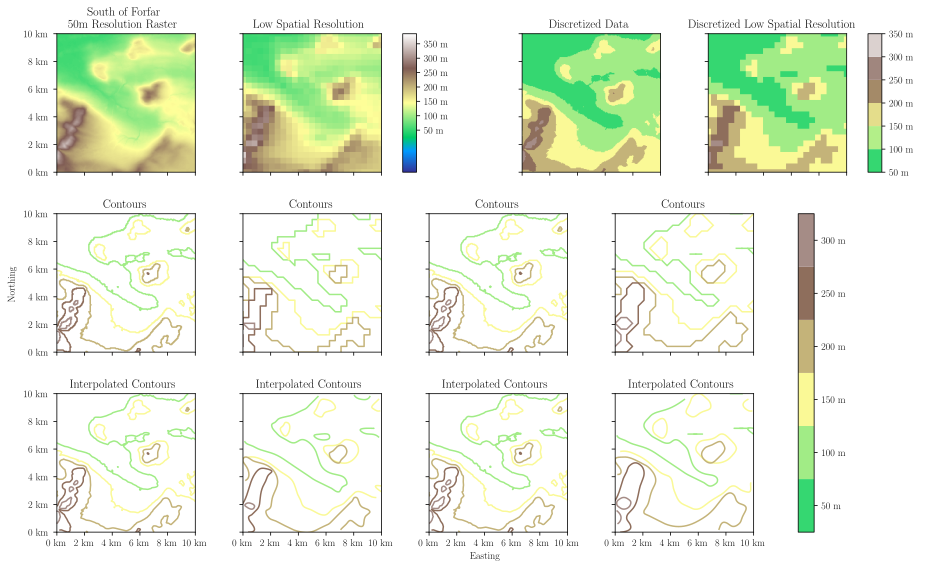
\includegraphics[width=1\textwidth]{../images/NO44/2D_Contour_Interpolation.png}
 % 2D_Contour_Interpolation.png: 1600x900 px, 100dpi, 40.64x22.86 cm, bb=0 0 1152 648
 \label{fig:2D_contour}
 \caption{Contour interpolation from data with various resolution.}
\end{figure}


\end{document}
